impetus\protect\index{Sachverzeichnis}{impetus} crescere  aequaliter, in quolibet puncto lineae tendentiae\protect\index{Sachverzeichnis}{linea  tendentiae}, hinc sequitur: tempora ad spatia percurrenda  necessaria, continue decrescere, et \edtext{quidem}{\lemma{}\Afootnote{\textit{Am Rand}: Ut conatus \protect\index{Sachverzeichnis}{conatus} crescunt in punctis, ita momenta decrescere in punctis.\vspace{-4mm}}} \edtext{momentum seu}{\lemma{momentum}\Bfootnote{\textit{(1)}\ quo percurritur \textit{(2)}\ seu \textit{L}\ }} tempus minus quolibet dato necessarium ad percurrendum punctum \textit{a} seu spatium minus quolibet dato, \edtext{esse ad momentum}{\lemma{esse}\Bfootnote{\textit{(1)}\ ut \textit{aa}, \textit{a}, vel \textit{pb} ad \textit{(2)}\ ad momentum \textit{L}\ }} quo percurrendum est punctum \edtext{\textit{c} ut est \textit{bb}, \textit{pp} ad \textit{hh}, \textit{oo}}{\lemma{\textit{c} ut est}\Bfootnote{%
\textit{(1)}\ \textit{aa}, \textit{a}, ad \textit{cc}, \textit{c}, seu %
\textit{(2)}\ \textit{bb}, \textit{pp} ad \textit{hh}, \textit{oo} \textit{L}}}
ut est \textit{pb} ad \textit{oh}.
Porro cum tempus quo percurritur spatium\protect\index{Sachverzeichnis}{spatium percursum} minus quolibet dato
\edtext{seu instans}{\lemma{seu}\Bfootnote{%
\textit{(1)}\ momentum %
\textit{(2)}\ instans \textit{erg. L}}}
exhibendum sit linea
\edtext{(\phantom)\hspace{-1.2mm}nam conatus}{\lemma{(nam\phantom)\hspace{-1.2mm}}\Bfootnote{%
\textbar\ si \textit{gestr.} \textbar\ conatus \textit{L}}}
exhibentur
\edtext{linea, et instantia}{\lemma{linea, et}\Bfootnote{\textit{(1)}\ tempora \textit{(2)}\ instantia \textit{L}}}
assumtis
\edtext{aequalibus punctis}{\lemma{aequalibus}\Bfootnote{\textit{(1)}\ spatiis \textit{(2)}\ punctis \textit{L}}}
habent, contrariam rationem conatuum\phantom(\hspace{-1.2mm}),
erit tempus quo percurritur linea \textit{ab}
\edtext{repraesentandum triangulo \textit{bb}, \textit{pp}, \textit{aa}}{\lemma{repraesentandum}\Bfootnote{%
\textit{(1)}\ linea \textit{(2)}\ triangulo %
\textit{(a)}\ \textit{aa}, \textit{a}, \textit{p}. %
\textit{(b)}\ \textit{bb}, \textit{pp}, \textit{aa} \textit{L}}}
seu \textit{bpa} et tempus quo percurritur linea \textit{cb} triangulo \textit{hoa}.
\edtext{Jam Trianguli}{\lemma{Jam}\Bfootnote{%
\textit{(1)}\ tempora %
\textit{(2)}\ Trianguli \textit{L}}}
sunt ut quadrata altitudinum,
\edtext{ergo duae lineae tendentiae,}{\lemma{ergo}\Bfootnote{%
\textit{(1)}\ spatio %
\textit{(2)}\ duae lineae tendentiae, \textit{L}}} eundem 
habentes terminum
\edtext{communem percurruntur temporibus quae sunt inter se, ut earum linearum quadrata.}{\lemma{communem}\Bfootnote{%
\textit{(1)}\ sunt inter se, ut qua %
\textit{(2)}\ percurruntur [...] quadrata. \textit{L}}}
Si ergo linea \textit{ab} divisa intelligatur
\edtext{in 7.}{\lemma{in}\Bfootnote{%
\textit{(1)}\ 8. %
\textit{(2)}\ 7. \textit{L}}}
partes, \textit{ac}. \textit{cd}. \textit{de}. \textit{ef}. \textit{fg}. \textit{gh}.
et \textit{hb}. percursa intelligatur tempore ut 1.
seu minuto  secundo 1. linea \textit{bg}. percursa erit minutis secundis 4.
\edtext{et \textit{bf} 2dis}{\lemma{et \textit{bf}}\Bfootnote{%
\textit{(1)}\ minutis %
\textit{(2)}\ 2dis \textit{L}}}
9. et \textit{be}. secundis 16. et \textit{bd} sec. 25. et \textit{bc} secundis 36. et \textit{ba} sec. 49.
Ergo linea \textit{ac}. percurretur secundis
\edtext{$49-36=13.$
Est enim differentia inter \textit{ba} 49. et \textit{bc} 36.
Et linea \textit{cd} sec. $36-25=11.$}{\lemma{$49-36=13.$}\Bfootnote{%
\textit{(1)}\ et linea \textit{cd}. sec. $36\,-$ %
\textit{(2)}\ Est enim [...] $36-25=11.$ \textit{L}}}
et linea \textit{de} 9. et \textit{ef} 7. et \textit{fg} 5. et \textit{gh} 3. et \textit{hb}. 1.
\pend 
\pstart Porro \edtext{ut instantia decrescunt, in datis aequalibus spatii punctis; ita spatii puncta crescunt}{\lemma{ut}\Bfootnote{%
\textit{(1)}\ tempora %
\textit{(2)}\ instantia \textbar\ aequaliter \textit{gestr.} \textbar\ decrescunt, %
\textit{(a)}\ ita spatia decursa decrescunt %
\textit{(b)}\ in %
\textit{(aa)}\ dato spatio %
\textit{(bb)}\ datis [...] ita %
\textit{(aaa)}\ spatia percurs %
\textit{(bbb)}\ spatii puncta crescunt \textit{L}}}
in datis aequalibus temporis instantibus.
Ergo punctum decurrendum instanti \textit{c} ad punctum decurrendum instanti \textit{d} est ut \textit{ci} ad \textit{dk}, et ita porro;
\edtext{ergo linea tendentiae percursa}{\lemma{ergo}\Bfootnote{\textit{(1)}\ spatium \textit{(2)}\ linea tendentiae percursa \textit{L}\ }}
tempore \textit{ac}
\edtext{ad percursam}{\lemma{$ac$ 
ad}\Bfootnote{\textit{(1)}\ spatium percursum \textit{(2)}\ percursam \textit{L}\ }}
tempore \textit{ad} est ut triangulum \textit{aci} ad triangulum \textit{adk} et
\edtext{proinde lineae temporibus inde a primo lapsus momento assumtis percursae sunt inter se ut}{\lemma{proinde}\Bfootnote{%
\textit{(1)}\ spatia %
\textit{(2)}\ ab eodem moti %
\textit{(3)}\ lineae tendentiae %
\textit{(a)}\ ab in %
\textit{(b)}\ inde ab initio %
\textit{(aa)} motus %
\textit{(bb)} decensus assumtae sunt inter se ut line %
\textit{(4)}\ lineae [...] inter se ut \textit{L}}}
quadrata temporum et lineae aequalibus temporibus percursae, sunt inter se ut numeri impares deinceps ab unitates seu differentiae quadratorum.
\pend
\vspace{2em} 
\pstart \noindent
\lbrack \textit{Nachfolgend klein gedruckter Text gestrichen:}\rbrack \pend 
\vspace{0.5em} 
\pstart 
\footnotesize
Ex his intelligitur nihil referre in prima nostra assumtione, an dicamus grave\protect\index{Sachverzeichnis}{grave} in quolibet lineae tendentiae\protect\index{Sachverzeichnis}{linea tendentiae} puncto, an in quolibet temporis descensus momento, novum accipere impetum\protect\index{Sachverzeichnis}{impetus}. Sed quaeritur an non impetus novi, in tempore potius quam loco sint computandi; computemus in tempore, videamusque quid inde \edtext{sequatur.%
\newline%
\indent%
In eadem quae supra est, figura $ab$ putetur esse tempus.}{\lemma{sequatur.}\Bfootnote{%
\textit{(1)}\ Esto tempus descensus $ab$. %
\textit{(2)}\ In eadem [...] tempus. %
\textbar\ Porro hoc supposito \textit{gestr.} \textbar\ \textit{L}}}
\pend 
\newpage
\pstart
\centering
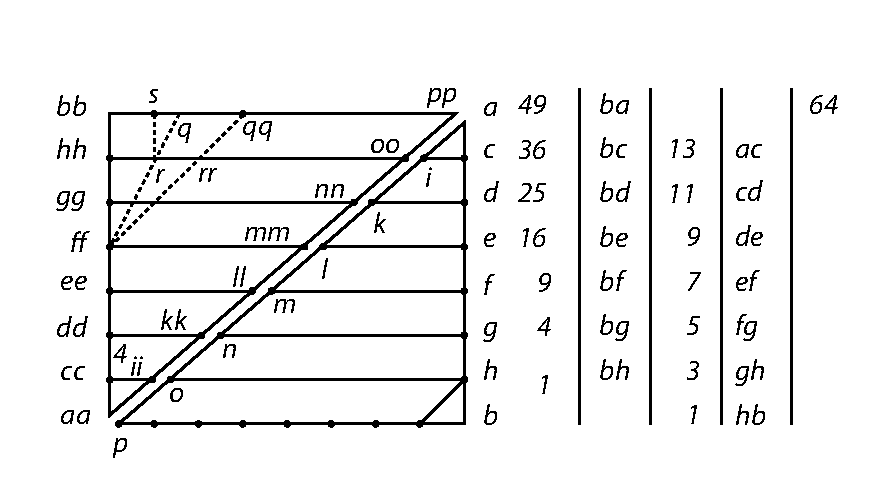
\includegraphics[trim = 0mm 5mm 0mm 10mm, clip,width=0.75\textwidth]{images/lh03705_128v-d1.pdf}\\
\noindent \centering [\textit{Fig. 2}] 
%\begin{minipage}[t]{0.5\textwidth}
%%\hspace*{-15mm}
%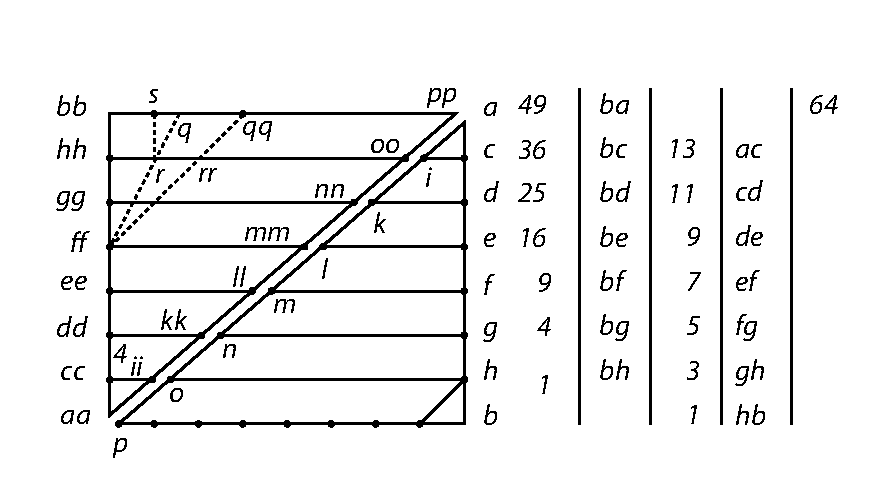
\includegraphics[width=1\textwidth]{images/lh03705_128v-d1.pdf}
%%\noindent \centering [\textit{Fig. 2}] 
%\end{minipage}
%%\hspace*{9,0mm}
%\begin{minipage}[t]{0.5\textwidth}
%\includegraphics[width=0.6\textwidth]{images/lh03705_128v-d2.pdf}\\
%%\noindent \centering [\textit{Fig. 3, gestrichen}] 
%\end{minipage}
%    \vspace*{5mm}
\pend 
\vspace*{1em}
\pstart
\centering
\includegraphics[width=0.4\textwidth]{images/lh03705_128v-d2.pdf}\\
\noindent \centering [\textit{Fig. 3, gestrichen}] 
\pend
\vspace{1.5em}
\count\Afootins=1200
\count\Bfootins=1000
\count\Cfootins=1200
\pstart
\noindent%
Si \setline{1}lineas assumas diversas, ex summo \textit{a} vel \textit{bb.}
\edtext{ut lineam \textit{ac}}{\lemma{ut lineam}\Bfootnote{%
\textit{(1)}\ \textit{bb} %
\textit{(2)}\ \textit{ac} \textit{L}}}
(\textit{bb}, \textit{hh}) ad lineam \textit{ae} (\textit{bb}, \textit{ff})
erunt tempora percursionis ut trapezium \textit{bpho}
\edtext{ad trapezium \textit{bpfm.} $BH$ minor, \textit{$BHF$} major, vel cum linea $bf$ major possit}%
{\lemma{ad trapezium \textit{bpfm.}}\Bfootnote{%
\textit{(1)}\ investigemus universaliter horum Trapeziorum rationem %
\textit{(2)}\ linea \textit{BP} arbitraria est, \textit{BH} et \textit{BF} datae quaelibet, Trapezium t %
\textit{(3)}\ $BH$ minor, %
\textit{(a)}\ \textit{BF} major %
\textit{(b)}\ \textit{BHF} major, %
\textit{(aa)}\ Trapezium \textit{bpho} est %
\textit{(bb)}\ \textit{HO} est ita ad \textit{ab} %
\textit{(cc)}\ vel cum linea $bf$ %
\textbar\ major \textit{erg.} \textbar\ possit \textit{L}}}
assumi pro tota linea descensus
(si ponas, grave\protect\index{Sachverzeichnis}{grave} in \textit{f} quiescere)
ut Trapezium \textit{bhqr} ad Triangulum \textit{bqf.}
\edtext{Jam \textit{BQ}}{\lemma{Jam}\Bfootnote{\textit{(1)}\ \textit{bq} \textit{(2)}\ \textit{BQ} \textit{L}}}
arbitraria est, \textit{BH} et \textit{BF}
\edtext{datae. $HR$}{\lemma{datae.}\Bfootnote{\textit{(1)}\ $HB$ \textit{(2)}\ $HR$ \textit{L}}}
\rule[-4mm]{0mm}{10mm}%
\edtext{est ad \textit{BQ} ut \textit{FB} ad $FH.$ $\displaystyle\frac{BQ}{HR}=\frac{FB}{FH}$ seu}%
{\lemma{est ad}\Bfootnote{%
\textit{(1)}\ \textit{bq} %
\textit{(2)}\ \textit{BQ} ut \textit{FB} ad %
\textit{(a)}\ \textit{HB.} %
\textit{(b)}\ \textit{FH.} %
\textit{(aa)}\ seu \textit{HR.} %
\textit{(bb)}\ $\displaystyle\frac{BQ}{HR}=\frac{FB}{FH}$ seu \textit{L}}}
\rule[-4mm]{0mm}{10mm}%
$\displaystyle \frac{HR}{BQ}=\frac{FH}{FB}.$
Ergo $\displaystyle HR=\frac{FH\smallfrown BQ}{FB}.$
\pend%
\newpage%
\pstart%
\noindent%
Triangulum \textit{bqf} est $\displaystyle\frac{BQ,\smallfrown BF}{2}$.
Jam Trapezium \textit{bhrq} componitur ex Rectangulo \textit{bhrs}, et Triangulo \textit{rqs.}
\rule[-4mm]{0mm}{10mm}Rectangulum est $\displaystyle FB-FH,\smallfrown HR$ seu
$\displaystyle FB\smallfrown\frac{FH\smallfrown BQ}{FB} - \displaystyle FH\smallfrown\frac{FH\smallfrown BQ}{FB}$, seu
\rule[-4mm]{0mm}{10mm}$\displaystyle FH\smallfrown BQ-FH^{2}\smallfrown\frac{BQ}{FB}$ seu $\displaystyle FH,,\smallfrown BQ,-FH\smallfrown \frac{BQ}{FB}$.
\edtext{Triangulum \textit{rqs} est:}{\lemma{Triangulum \textit{rqs} est:}\Bfootnote{\textit{erg. L}}}
$\displaystyle FB-FH.\smallfrown BQ-\frac{FH\smallfrown BQ}{FB},\, + \, \dots \rule[-4mm]{0mm}{10mm}$
\edtext{Trapezium}{\lemma{Trapezium}\Bfootnote{\textit{erg. L}}}
$\displaystyle FB\smallfrown BQ,\smallfrown \frac{FH,\smallfrown BQ}{3},,2+FH^{2}\frac{BQ}{FB}.$
Et hujus ratio ad Triangulum \textit{bqf} est
(sublato ubique \textit{BQ})
quae \rule[-4mm]{0mm}{10mm}$\displaystyle FB-\frac{FH}{3}+\frac{FH^{2}}{FB}$ ad $\displaystyle \frac{BF}{2}$
seu ut $\displaystyle 1+\frac{FH^{2}}{FB^{2}}-\frac{FH}{3BF}$ ad $\displaystyle \frac {1}{2}$
seu Ratio est: \rule[-4mm]{0mm}{10mm}$\displaystyle\frac{1}{2}+\frac{FH^{2}}{2FB^{2}}-\frac{FH}{3BF}.$
Ergo si Triangulum est 1. Trapezium est
\rule[-4mm]{0mm}{10mm}%
$\displaystyle\frac{1}{2}+\frac{FH^{2}}{2FB^{2}}-\frac{FH}{3BF}.$
[129~r\textsuperscript{o}]%
\pend